\documentclass[letterpaper,11pt,titlepage,draftclsnofoot,onecolumn,compsoc,utf8,latin1]{IEEEtran}
\usepackage{graphicx}
\usepackage{amssymb}
\usepackage{amsmath}
\usepackage{array}
\usepackage{amsthm}
\usepackage{listings}
\usepackage{alltt}
\usepackage{float}
\usepackage{color}
\usepackage{url}
\usepackage{setspace}
\usepackage{balance}
\usepackage{enumitem}
\usepackage{pstricks, pst-node}
\usepackage{inputenc}
\usepackage[margin=.75in]{geometry}
\usepackage{courier}
\usepackage{fancyhdr}
\usepackage{hyperref}
\usepackage{geometry}
\usepackage{tocloft}
\usepackage{tabu}

%crappy error with titlesec
\newcommand{\subparagraph}{}
\usepackage{titlesec}
\setlength{\parindent}{.25in}

\lstset
{ %Formatting for code in appendix
    %frame=single,
    basicstyle=\footnotesize\ttfamily,
    numbers=left,
    numbersep=.25in,
    stepnumber=1,
    showstringspaces=false,
    tabsize=4,
    breakatwhitespace=false,
    xleftmargin=.5in,
    xrightmargin=.5in,
}

%toc formatting for IEEE 830-1998 standards
\renewcommand{\cftsecleader}{\cftdotfill{\cftdotsep}{\vspace{.25cm}}}
\renewcommand{\cftsecfont}{\normalfont}
\renewcommand{\cftsecpagefont}{\normalfont}
\renewcommand{\cftsecaftersnum}{.}

%formatting specific IEEE 830-1998 Section headings
\titleformat{\section}[block]
  {\fontsize{12}{12}\bfseries\sffamily}
  {\thesection.}
  {1em}
  {}
\titleformat{\subsection}[block]
  {\fontsize{12}{12}\bfseries\sffamily}
  {\thesubsection}
  {1em}
  {\vspace{.1cm}}
\titleformat{\subsubsection}[block]
  {\fontsize{12}{12}\bfseries\sffamily}
  {\thesubsubsection}
  {1em}
  {\vspace{.2cm}}
  
\newcommand{\cred}[1]{{\color{red}#1}}
\newcommand{\cblue}[1]{{\color{blue}#1}}

\def\name{Charles Siebert}
\def\mytitle{Final Project}
\def\myemail{siebertc@oregonstate.edu}

%% The following metadata will show up in the PDF properties
\hypersetup{
  pdfauthor = {\name},
  pdfkeywords = {cs493 "Final"},
  pdftitle = {\mytitle},
  pdfsubject = {CS 493 Final},
  pdfpagemode = UseNone
}

\begin{document}
\begin{titlepage}
\centering
\vspace*{9cm}
{\scshape\LARGE \mytitle} \\
	{\scshape\Large CS493 - Fall 2019 \par}
	\vspace{.5cm}
	{\large{\bfseries Author:} \name} \par
	{\large{\bfseries E-mail:} \myemail} \par
    {\large \today \par} 
    {\large https://siebertc-cs493-final.appspot.com/ \par} 
	\vspace*{1cm}

\end{titlepage}

\newpage

\thispagestyle{empty}
\pagenumbering{gobble}

\tableofcontents

\cleardoublepage
\pagenumbering{arabic}

\newpage

\begin{singlespace}

\section{Introduction}
This is the Final Project for CS493, where we put together all aspects of what we've learned in class, along with authorization on protected resources, and deployed on Google Cloud Platform (GCP). In this project, we're to allow the creation of accounts, and authenticate to protected resources on our RESTful API design. Access to my Project is found at https://siebertc-cs493-final.appspot.com/ \\

\noindent
The rest of this document outlines the endpoints required for Homework 4, with some tweaks to fit the requirements that were otherwise specified in the Final Project outline. The base web page is taken from my Google OAuth2.0 project, that endpoint isn't implemented and has a useless button that goes to an endpoint that doesn't exist. After signing in with Google OAuth2.0, a user entity is automatically generated.

\subsection{Account Creation}
To create a user account, you will go to https://siebertc-cs493-final.appspot.com/ and there will be a "submit" button that will open a third party page to authenticate with Google Auth2.0 and after successfully returning back to my webpage, it will display your \textbf{jwt} along with the \textbf{sub} property to uniquely identify you with your user account. Please see the below picture to see an example transition when using my account creation.

\begin{center}
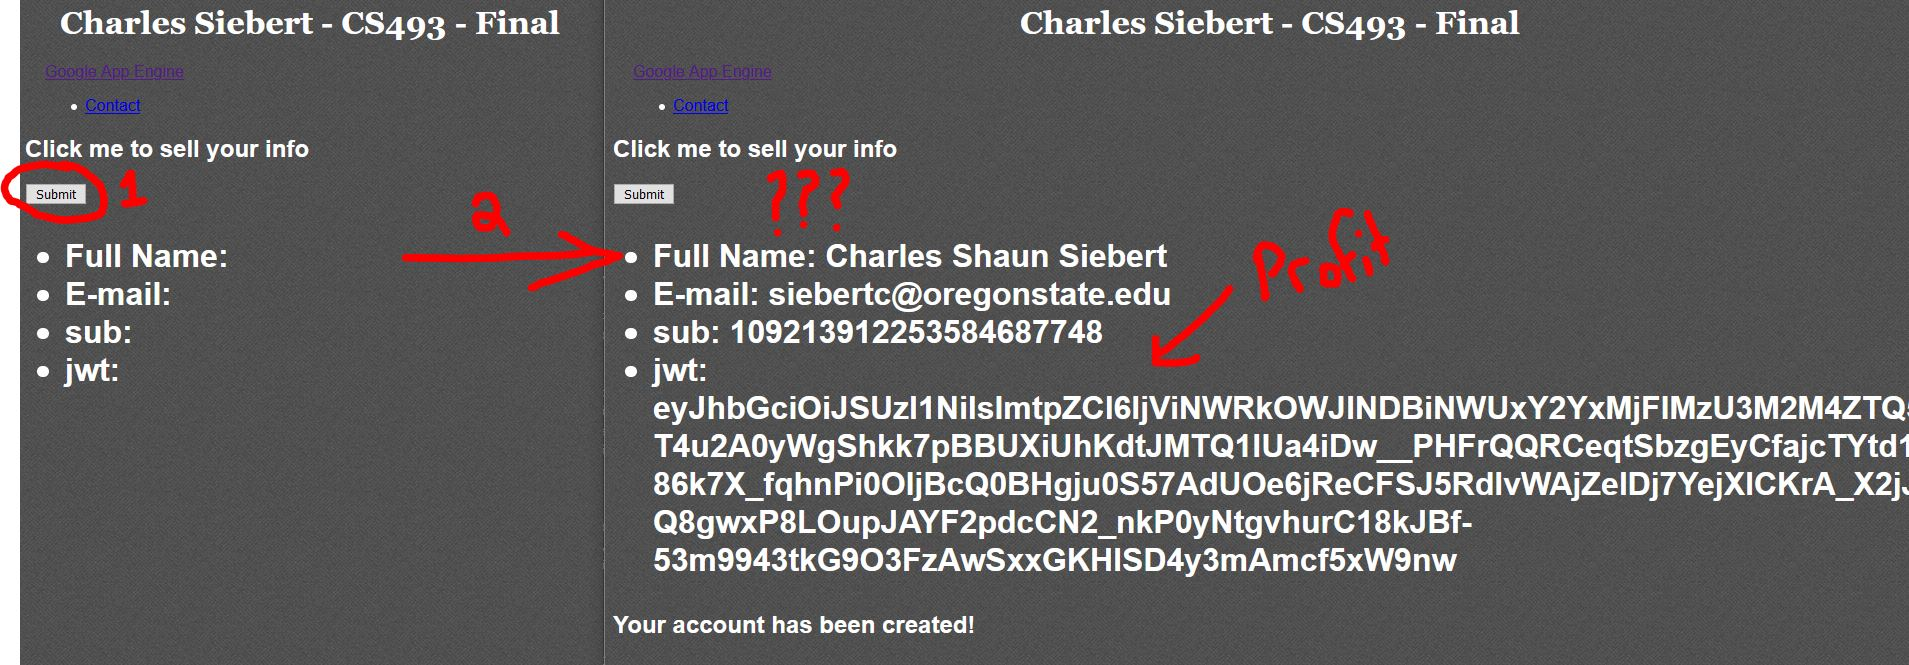
\includegraphics[width=\textwidth]{accountcreation.JPG}\\
\caption{\textbf{Figure 1. } Transitions on my homepage detailing account creation.}\\
\end{center}

\subsection{Relational Schema}
Please see the attached picture of a relational schema that is used to model the data relationships that is stored in the NoSQL Datastore used in my GCP project. The user identity is used by Google OAuth2.0 in the \textbf{sub} property, so while our NoSQL Datastore creates unique IDs specifically within itself as shown by the \textbf{id} in the following schemas, the \textbf{sub} property is a unique ID that is given by Google as a unique identifier. I use this property to check for user accounts and identify who owns what boats.

\begin{center}
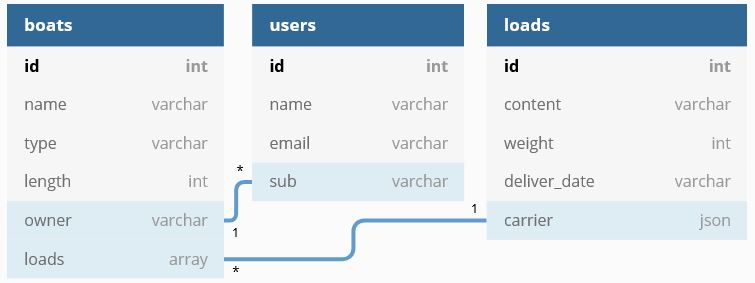
\includegraphics[width=.8\textwidth]{relationalschema.JPG}\\
\caption{\textbf{Figure 2. } Diagram showing relationships between all three entities.}\\
\end{center}

\subsection{Authentication}
There are JWT authentications at the following endpoints: Create Boat, edit boat, delete boat, delete load, add load to a boat, and remove load from a boat. \\

The test requires TWO JWT tokens. I've made a spare gmail account for you to use\\
Username: siebertccs493final@gmail.com\\
Password: SuperSecretPassword123\\

JWT tokens go into the environment variables jwt1 and jwt2\\

\subsection{Other unfinished sections}
Here's the considerations for sections I couldnt finish in time. I've worked on editing loads and boats, where specifically boats need user authentication for editing them. I've managed to get patching working, but never did a check for who was doing the edits. Along with all of the endpoints and the status codes, the documentation hasn't been fully updated. All testing should show the status codes of: 200, 201, 204, 401, 403, 405, and 406 on some endpoints. Please look at those.\\

\section{Create a User}

Allows you to create a new user\\

\noindent \textbf{POST} /boats

\subsection{Request}

\subsubsection{Request Parameters}

Authentication: 'Bearer' + JWT

\subsubsection{Request Body}


\subsubsection{Request Body Format}

JSON

\subsection{Response}
\subsubsection{Response Body Format}

JSON

\subsubsection{Response Statuses}

\begin{center}
\begin{tabular}{ |p{.2\textwidth}|p{.2\textwidth}|p{.52\textwidth}| } 
 \hline
 \textbf{Outcome} & \textbf{Status Code} & \textbf{Notes}  \\  \hline
 Success & 201 Created &  \\ 
 \hline
\end{tabular}
\end{center}

\subsubsection{Response Examples}

Datastore will automatically generate an ID and store it with the entity being created.This value needs to be sent in the response body as shown in the example.\\

\noindent The \texttt{self} attribute will contain the live link to the REST resource corresponding to this boat. In other words, this is the URL to get this newly created boat. You must not store the self attribute in Datastore.\\

\noindent The \texttt{self} attribute will contain the live link to the REST resource corresponding to the loads the boat has. In other words, this is the URL to get the loads on the boat. You must not store the self attribute in Datastore.\\

\noindent \Large{Success}

\begin{lstlisting}[]
Status: 201 Created
{
    "id": "abc123",
    "name": "Charles Shaun Siebert",
    "email": "siebertc@oregonstate.edu",
    "sub": 1234567890,
    "self": "https://<your-app>/users/abc123"
}
\end{lstlisting}

\newpage 

\normalsize

\section{View a User}

Allows you to view an existing user\\

\noindent \textbf{GET} /boats/:user\_id

\subsection{Request}

\subsubsection{Request Parameters}

\begin{center}
    \begin{tabular}{ | p{.1\textwidth} | p{.1\textwidth} | p{.6\textwidth} | p{.1\textwidth} |}
    \hline
        \textbf{Name} & \textbf{Type} & \textbf{Description} &\textbf{Required?}  \\ \hline
        user\_id & String & ID of the user & Yes \\
    \hline
    \end{tabular}
\end{center}

\subsubsection{Request Body}

None

\subsection{Response}
\subsubsection{Response Body Format}

JSON

\subsubsection{Response Statuses}

\begin{center}
\begin{tabular}{ |p{.2\textwidth}|p{.2\textwidth}|p{.52\textwidth}| } 
 \hline
 \textbf{Outcome} & \textbf{Status Code} & \textbf{Notes}  \\  \hline
 Success & 200 OK &  \\ \hline
 Failure & 404 Not Found & No user with this user\_id exists \\ \hline
 \hline
\end{tabular}
\end{center}

\subsubsection{Response Examples}

\noindent \Large{Success}

\begin{lstlisting}[]
Status: 200 OK
{
    "id": "abc123",
    "name": "Charles Shaun Siebert",
    "email": "siebertc@oregonstate.edu",
    "sub": 1234567890,
    "self": "https://<your-app>/users/abc123"
}
\end{lstlisting}

\noindent \Large{Failure}

\begin{lstlisting}[]
Status: 404 Failure
{
    "Error: "No user with this user_id exists"
}
\end{lstlisting}

\newpage 

\normalsize

\section{View all Users}

Allows you to view all existing users\\

\noindent \textbf{GET} /users

\subsection{Request}

\subsubsection{Request Parameters}

None

\subsubsection{Request Body}

None

\subsection{Response}

\subsubsection{Response Body Format}

JSON

\subsubsection{Response Statuses}

\begin{center}
\begin{tabular}{ |p{.2\textwidth}|p{.2\textwidth}|p{.52\textwidth}| } 
 \hline
 \textbf{Outcome} & \textbf{Status Code} & \textbf{Notes}  \\  \hline
 Success & 200 OK &  \\
 \hline
\end{tabular}
\end{center}

\subsubsection{Response Examples}

\noindent \Large{Success}

\begin{lstlisting}[]
Status: 200 OK

{
    "items": [
        {
            "id": "abc123",
            "name": "Charles Shaun Siebert",
            "email": "siebertc@oregonstate.edu",
            "sub": 1234567890,
            "self": "https://<your-app>/users/abc123"
        },
        {
            "id": "def456",
            "name": "Shaun Siebert",
            "email": "siebertcharles@oregonstate.edu",
            "sub": 12345678902342,
            "self": "https://<your-app>/users/def456"
        }
    ],
}
\end{lstlisting}

\newpage 


\section{Create a Boat}

Allows you to create a new boat\\

\noindent \textbf{POST} /boats

\subsection{Request}

\subsubsection{Request Parameters}

None

\subsubsection{Request Body}

Required

\subsubsection{Request Body Format}

JSON

\subsubsection{Request JSON Attributes}

\begin{center}
\begin{tabular}{ |p{.1\textwidth}|p{.1\textwidth}|p{.6\textwidth}|p{.1\textwidth}| } 
 \hline
 \textbf{Name} & \textbf{Type} & \textbf{Description} & \textbf{Required?} \\  \hline
 name & String & The name of the boat. & Yes  \\ \hline
 type & String & The type of the boat. E.g., Sailboat, catamaran, etc. & Yes \\ \hline 
 length & Integer & Length of the boat in feet. & Yes \\ 
 \hline
\end{tabular}
\end{center}

\subsubsection{Request Body Example}

\begin{lstlisting}[]
{
    "name": "Sea Witch",
    "type": "Catamaran",
    "length": 28
}
\end{lstlisting}

\subsection{Response}
\subsubsection{Response Body Format}

JSON

\subsubsection{Response Statuses}

\begin{center}
\begin{tabular}{ |p{.2\textwidth}|p{.2\textwidth}|p{.52\textwidth}| } 
 \hline
 \textbf{Outcome} & \textbf{Status Code} & \textbf{Notes}  \\  \hline
 Success & 201 Created &  \\ \hline
 Failure & 400 Bad Request &  
 If the request is missing any of the 3 required attributes, the boat must not be created,and 400 status code must be returned.\vspace{.2cm}
 You don’t need to validate the values of the attributes and can assume that if the request contains any of the listed attributes, then that attribute’s value is valid.\vspace{.2cm}
 You can also assume that the request will not contain any extraneous attribute (i.e., the request JSON will never contain any attribute other than the ones that are listed).\\ \hline
 Failure & 406 Bad Request & Server received incorrect content-type MIME in request body.\\
 \hline
\end{tabular}
\end{center}

\subsubsection{Response Examples}

Datastore will automatically generate an ID and store it with the entity being created.This value needs to be sent in the response body as shown in the example.\\

\noindent The \texttt{self} attribute will contain the live link to the REST resource corresponding to this boat. In other words, this is the URL to get this newly created boat. You must not store the self attribute in Datastore.\\

\noindent The \texttt{self} attribute will contain the live link to the REST resource corresponding to the loads the boat has. In other words, this is the URL to get the loads on the boat. You must not store the self attribute in Datastore.\\

\noindent \Large{Success}

\begin{lstlisting}[]
Status: 201 Created
{
    "id": "abc123",
    "name": "Sea Witch",
    "type": "Catamaran",
    "length": 28,
    "loads": null,
    "owner": 123456790,
    "self": "https://<your-app>/boats/abc123"
}
\end{lstlisting}

\noindent \Large{Failure}

\begin{lstlisting}[]
Status: 400 Bad Request
{
    "Error: "The request object is missing at least one of the required attributes"
}
\end{lstlisting}

\noindent \Large{Failure}

\begin{lstlisting}[]
Status: 406 Bad Request
{
    "Error: "The server only accepts application/json data."
}
\end{lstlisting}

\newpage 

\normalsize

\section{View a Boat}

Allows you to view an existing boat\\

\noindent \textbf{GET} /boats/:boat\_id

\subsection{Request}

\subsubsection{Request Parameters}

\begin{center}
    \begin{tabular}{ | p{.1\textwidth} | p{.1\textwidth} | p{.6\textwidth} | p{.1\textwidth} |}
    \hline
        \textbf{Name} & \textbf{Type} & \textbf{Description} &\textbf{Required?}  \\ \hline
        boat\_id & String & ID of the boat & Yes \\
    \hline
    \end{tabular}
\end{center}

\subsubsection{Request Body}

None

\subsection{Response}
\subsubsection{Response Body Format}

JSON

\subsubsection{Response Statuses}

\begin{center}
\begin{tabular}{ |p{.2\textwidth}|p{.2\textwidth}|p{.52\textwidth}| } 
 \hline
 \textbf{Outcome} & \textbf{Status Code} & \textbf{Notes}  \\  \hline
 Success & 200 OK &  \\ \hline
 Failure & 404 Not Found & No boat with this boat\_id exists \\ \hline
 \hline
\end{tabular}
\end{center}

\subsubsection{Response Examples}

\noindent \Large{Success}

\begin{lstlisting}[]
Status: 200 OK
{
    "id": "abc123",
    "name": "Sea Witch",
    "type": "Catamaran",
    "length": 28,
    "owner": 123456790,
    "loads": [
        {
            "id": "123abc",
            "self": "https://<your-app>/loads/123abc"
        }
    ]
    "self": "https://<your-app>/boats/abc123"
}
\end{lstlisting}

\noindent \Large{Failure}

\begin{lstlisting}[]
Status: 404 Failure
{
    "Error: "No boat with this boat_id exists"
}
\end{lstlisting}

\newpage 

\normalsize

\section{View all Boats}

Allows you to view all existing boats. Implements pagination, every three boats.\\

\noindent \textbf{GET} /boats

\subsection{Request}

\subsubsection{Request Parameters}

None

\subsubsection{Request Body}

None

\subsection{Response}

\subsubsection{Response Body Format}

JSON

\subsubsection{Response Statuses}

\begin{center}
\begin{tabular}{ |p{.2\textwidth}|p{.2\textwidth}|p{.52\textwidth}| } 
 \hline
 \textbf{Outcome} & \textbf{Status Code} & \textbf{Notes}  \\  \hline
 Success & 200 OK &  \\
 \hline
\end{tabular}
\end{center}

\subsubsection{Response Examples}

\noindent \Large{Success}

\begin{lstlisting}[]
Status: 200 OK

{
    "items": [
        {
            "type": "Yatch",
            "loads": null,
            "length": 99,
            "name": "Odyssey",
            "id": "4787714943614976",
            "owner": 123456790,
            "self": "https://siebertc-cs493-hw4.appspot.com/boats/4787714943614976"
        },
        {
            "type": "Yatch",
            "loads": null,
            "length": 99,
            "name": "Odyssey",
            "id": "4823100818456576",
            "owner": 123456790,
            "self": "https://siebertc-cs493-hw4.appspot.com/boats/4823100818456576"
        },
        {
            "length": 99,
            "name": "Odyssey",
            "type": "Yatch",
            "loads": null,
            "id": "5172860540682240",
            "owner": 123456790,
            "self": "https://siebertc-cs493-hw4.appspot.com/boats/5172860540682240"
        }
    ],
    "next": "https://siebertc-cs493-hw4.appspot.com/boats?cursor=Ci8SKWoUbX5zaWViZXJ0Yy1jczQ5My1odzRyEQsSBEJvYXQYgICAmIeWmAkMGAAgAA=="
}
\end{lstlisting}

\newpage 

\normalsize

\section{Delete a Boat}

Allows you to delete a boat. Note that if the boat is currently holding a load, deleting the boat makes the carrier field on the load become the default null value. The load has no carrier after the boat is holding it is deleted.\\

\noindent \textbf{DELETE} /boats/:boat\_id

\subsection{Request}

\subsubsection{Request Parameters}

\begin{center}
    \begin{tabular}{ | p{.1\textwidth} | p{.1\textwidth} | p{.6\textwidth} | p{.1\textwidth} |}
    \hline
        \textbf{Name} & \textbf{Type} & \textbf{Description} &\textbf{Required?}  \\ \hline
        boat\_id & String & ID of the boat & Yes \\
    \hline
    \end{tabular}
\end{center}

\subsubsection{Request Body}

None

\subsection{Response}

No Body

\subsubsection{Response Body Format}
Success: No Body\\
\noindent Failure: JSON

\subsubsection{Response Statuses}

\begin{center}
\begin{tabular}{ |p{.2\textwidth}|p{.2\textwidth}|p{.52\textwidth}| } 
 \hline
 \textbf{Outcome} & \textbf{Status Code} & \textbf{Notes}  \\  \hline
 Success & 204 No Content &  \\ \hline
 Failure & 404 Not Found & No boat with this boat\_id exists \\
 \hline
\end{tabular}
\end{center}

\subsubsection{Response Examples}

\noindent \Large{Success}

\begin{lstlisting}[]
Status: 204 No Content
\end{lstlisting}

\noindent \Large{Failure}

\begin{lstlisting}[]
Status: 404 Failure
{
    "Error: "No boat with this boat_id exists"
}
\end{lstlisting}

\begin{lstlisting}[]
Status: 403 Forbidden
{
    "Error": "You do not have access to edit this entity."
}
\end{lstlisting}

\newpage

\normalsize

\section{Delete a Boat #2}

Allows you to delete a boat. Note this is on the root of "boats". We need to always return an error on this type of request.\\

\noindent \textbf{DELETE} /boats

\subsection{Request}

\subsubsection{Request Body}

None

\subsection{Response}

No Body

\subsubsection{Response Body Format}

No response

\subsubsection{Response Statuses}

\begin{center}
\begin{tabular}{ |p{.2\textwidth}|p{.2\textwidth}|p{.52\textwidth}| } 
 \hline
 \textbf{Outcome} & \textbf{Status Code} & \textbf{Notes}  \\  \hline
 Failure & 405 Method Not Allowed & The method calling on this folder isn't allowed, and returns an error \\
 \hline
\end{tabular}
\end{center}

\newpage

\normalsize

\section{Edit a Boat}

Allows you to edit a boat. The request body MUST have all three attributes.\\

\noindent \textbf{PATCH} /boats/:boat\_id

\subsection{MIME Type}

application/json

\subsection{Request}

\subsubsection{Request Parameters}

\begin{center}
    \begin{tabular}{ | p{.1\textwidth} | p{.1\textwidth} | p{.6\textwidth} | p{.1\textwidth} |}
    \hline
        \textbf{Name} & \textbf{Type} & \textbf{Description} &\textbf{Required?}  \\ \hline
        boat\_id & String & ID of the boat & Yes \\
    \hline
    \end{tabular}
\end{center}
\subsubsection{Request Body}

Required

\subsubsection{Request Body Format}

JSON

\subsubsection{Request JSON Attributes}

\begin{center}
\begin{tabular}{ |p{.1\textwidth}|p{.1\textwidth}|p{.6\textwidth}|p{.1\textwidth}| } 
 \hline
 \textbf{Name} & \textbf{Type} & \textbf{Description} & \textbf{Required?} \\  \hline
 name & String & The name of the boat. & No  \\ \hline
 type & String & The type of the boat. E.g., Sailboat, catamaran, etc. & No \\ \hline 
 length & Integer & Length of the boat in feet. & No \\ 
 \hline
\end{tabular}
\end{center}

\subsubsection{Request Body Example}

\begin{lstlisting}[]
{
    "name": "Sea Witch",
    "type": "Catamaran",
    "length": 28
}
\end{lstlisting}

\subsection{Response}
\subsubsection{Response Body Format}

JSON

\subsubsection{Response Statuses}

\begin{center}
\begin{tabular}{ |p{.2\textwidth}|p{.2\textwidth}|p{.52\textwidth}| } 
 \hline
 \textbf{Outcome} & \textbf{Status Code} & \textbf{Notes}  \\  \hline
 Success & 201 Successful & \\ \hline
 Failure & 400 Bad Request &  
 If the request is missing any of the 3 required attributes, the boat must not be updated, and 400 status code must be returned.\\ \hline
 Failure & 403 Forbidden & You do not have access to edit this entity. \\ \hline
 Failure & 404 Not Found & No boat with this boat_exists \\ \hline
 Failure & 406 Not Acceptable & Content is not supported by this endpoint. \\
 \hline
\end{tabular}
\end{center}

\subsubsection{Response Examples}

When PUT is used to edit a boat, the response should return a 303 code with the location of the updated boat in the appropriate header field.

\noindent \Large{Success}

\begin{lstlisting}[]
Status: 201 Other Method
{
    "id": "abc123",
    "name": "Sea Witch",
    "type": "Catamaran",
    "length": 28,
    "owner": 123456790,
    "self": "https://<your-app>/boats/abc123"
}
\end{lstlisting}

\noindent \Large{Failure}

\begin{lstlisting}[]
Status: 400 Bad Request
{
    "Error: "The request object is missing at least one of the required attributes"
}
\end{lstlisting}

\begin{lstlisting}[]
Status: 403 Forbidden
{
    "Error": "You do not have access to edit this entity."
}
\end{lstlisting}

\begin{lstlisting}[]
Status: 404 Not Found
{
    "Error: "No boat with this boat_id exists"
}
\end{lstlisting}

\begin{lstlisting}[]
Status: 406 Not Acceptable
{
    "Error: "Server only accepts application/json data."
}
\end{lstlisting}

\newpage 

\normalsize

\section{Put a Boat}

Allows you to PUT a boat. Note this is on the root of "boats". We need to always return an error on this type of request.\\

\noindent \textbf{PUT} /boats

\subsection{Request}

\subsubsection{Request Body}

None

\subsection{Response}

No Body

\subsubsection{Response Body Format}

No response

\subsubsection{Response Statuses}

\begin{center}
\begin{tabular}{ |p{.2\textwidth}|p{.2\textwidth}|p{.52\textwidth}| } 
 \hline
 \textbf{Outcome} & \textbf{Status Code} & \textbf{Notes}  \\  \hline
 Failure & 405 Method Not Allowed & The method calling on this folder isn't allowed, and returns an error \\
 \hline
\end{tabular}
\end{center}

\newpage

\normalsize

\section{Create a Load}

Allows you to create a new load. A new load must not be assigned to a boat at time of creation.\\

\noindent \textbf{POST} /loads

\subsection{Request}

\subsubsection{Request Parameters}

None

\subsubsection{Request Body}

Required

\subsubsection{Request Body Format}

JSON

\subsubsection{Request JSON Attributes}

\begin{center}
\begin{tabular}{ |p{.15\textwidth}|p{.1\textwidth}|p{.55\textwidth}|p{.1\textwidth}| } 
 \hline
 \textbf{Name} & \textbf{Type} & \textbf{Description} & \textbf{Required?} \\  \hline
 weight & Integer & How much the load weighs & Yes  \\ \hline
 content & String & Name of the contents that the load is carrying & Yes \\ \hline 
 delivery\_date & String & Due date of the shipment & Yes \\
 \hline
\end{tabular}
\end{center}

\subsubsection{Request Body Example}

\begin{lstlisting}[]
{
    "weight": 5,
    "content": "LEGO Blocks",
    "delivery_date": "1/1/2020"
}
\end{lstlisting}

\subsection{Response}
\subsubsection{Response Body Format}

JSON

\subsubsection{Response Statuses}

\begin{center}
\begin{tabular}{ |p{.2\textwidth}|p{.2\textwidth}|p{.52\textwidth}| } 
 \hline
 \textbf{Outcome} & \textbf{Status Code} & \textbf{Notes}  \\  \hline
 Success & 201 Created &  \\ \hline
 Failure & 400 Bad Request &  
 If the request is missing any of the 3 required attributes, the load must not be created, and 400 status code must be returned.\vspace{.2cm}
 You don’t need to validate the values of the attributes and can assume that if the request contains any of the listed attributes, then that attribute’s value is valid.\vspace{.2cm}
 You can also assume that the request will not contain any extraneous attribute (i.e., the request JSON will never contain any attribute other than the ones that are listed).\\ \hline
  Failure & 406 Bad Request & Server received incorrect content-type MIME in request body. \\
 \hline
\end{tabular}
\end{center}

\subsubsection{Response Examples}

Datastore will automatically generate an ID and store it with the entity being created. This value needs to be sent in the response body as shown in the example.\\

\noindent The \texttt{self} attribute will contain the live link to the REST resource corresponding to this load. In other words, this is the URL to get this newly created load. You must not store the self attribute in Datastore.\\

\noindent \Large{Success}

\begin{lstlisting}[]
Status: 201 Created
{ 
    "id": "123abc", # automatically generated by the Datastore
    "weight": 5,     #The weight of the load
    "carrier": null,  #The boat carrying the load
    "content": "LEGO Blocks",
    "delivery_date": "1/1/2020" #The date the load is to be delivered
    "self": "https://appspot.com/loads/123abc"
}
\end{lstlisting}

\noindent \Large{Failure}

\begin{lstlisting}[]
Status: 400 Bad Request
{
    "Error: "The request object is missing at least one of the required attributes"
}
\end{lstlisting}

\noindent \Large{Failure}

\begin{lstlisting}[]
Status: 406 Bad Request
{
    "Error: "The server only accepts application/json data."
}
\end{lstlisting}


\newpage 

\normalsize

\section{View a Load}

Allows you to view an existing load\\

\noindent \textbf{GET} /loads/:load\_id

\subsection{Request}

\subsubsection{Request Parameters}

\begin{center}
    \begin{tabular}{ | p{.1\textwidth} | p{.1\textwidth} | p{.6\textwidth} | p{.1\textwidth} |}
    \hline
        \textbf{Name} & \textbf{Type} & \textbf{Description} &\textbf{Required?}  \\ \hline
        load\_id & String & ID of the load & Yes \\
    \hline
    \end{tabular}
\end{center}

\subsubsection{Request Body}

None

\subsection{Response}
\subsubsection{Response Body Format}

JSON

\subsubsection{Response Statuses}

\begin{center}
\begin{tabular}{ |p{.2\textwidth}|p{.2\textwidth}|p{.52\textwidth}| } 
 \hline
 \textbf{Outcome} & \textbf{Status Code} & \textbf{Notes}  \\  \hline
 Success & 200 OK &  \\ \hline
 Failure & 404 Not Found & No load with this load\_id exists \\
 \hline
\end{tabular}
\end{center}

\subsubsection{Response Examples}

\noindent \Large{Success}

\begin{lstlisting}[]
Status: 200 OK
{ 
    "id": "123abc",
    "weight": 5,
    "carrier": {
        "id": "abc123",
        "name": "Sea Witch"
        "self": https://<your-app>/boats/abc123
    },
    "content": "LEGO Blocks",
    "delivery_date": "1/1/2020"
    "self": "https://appspot.com/loads/123abc"
}
\end{lstlisting}

\noindent \Large{Failure}

\begin{lstlisting}[]
Status: 404 Failure
{
    "Error: "No load with this load_id exists"
}
\end{lstlisting}

\newpage

\normalsize

\section{View all Loads}

Allows you to view all existing loads. Implements pagination, every three boats.\\

\noindent \textbf{GET} /loads

\subsection{Request}

\subsubsection{Request Parameters}

None

\subsubsection{Request Body}

None

\subsection{Response}

\subsubsection{Response Body Format}

JSON

\subsubsection{Response Statuses}

\begin{center}
\begin{tabular}{ |p{.2\textwidth}|p{.2\textwidth}|p{.52\textwidth}| } 
 \hline
 \textbf{Outcome} & \textbf{Status Code} & \textbf{Notes}  \\  \hline
 Success & 200 OK &  \\
 \hline
\end{tabular}
\end{center}

\subsubsection{Response Examples}

\noindent \Large{Success}

\begin{lstlisting}[]
Status: 200 OK
{
    "items": [
        {
            "content": "LEGO Blocks",
            "weight": 1,
            "delivery_date": "1/1/2021",
            "carrier": {
                "name": "Odyssey",
                "id": "5740877414662144"
            },
            "id": "5112644562321408",
            "self": "https://siebertc-cs493-hw4.appspot.com/loads/5112644562321408"
        },
        {
            "carrier": {
                "name": "Odyssey",
                "id": "5951867817295872"
            },
            "content": "LEGO Blocks",
            "weight": 1,
            "delivery_date": "1/1/2021",
            "id": "5146163359514624",
            "self": "https://siebertc-cs493-hw4.appspot.com/loads/5146163359514624"
        },
        {
            "carrier": {
                "id": "5951867817295872",
                "name": "Odyssey"
            },
            "content": "LEGO Blocks",
            "weight": 1,
            "delivery_date": "1/1/2021",
            "id": "5424333895761920",
            "self": "https://siebertc-cs493-hw4.appspot.com/loads/5424333895761920"
        }
    ],
    "next": "https://siebertc-cs493-hw4.appspot.com/loads?cursor=Ci8SKWoUbX5zaWViZXJ0Yy1jczQ5My1odzRyEQsSBExvYWQYgICAuPKs0QkMGAAgAA=="
}
\end{lstlisting}

\newpage 

\normalsize

\section{Delete a Load}

Allows you to delete a load. Note that if the load is currently assigned to a boat, deleting the load makes the "loads" field on the boat become removed from the array. The boat no longer has the load information specific to the one that was just deleted.\\

\noindent \textbf{DELETE} /loads/:load\_id

\subsection{Request}

\subsubsection{Request Parameters}

\begin{center}
    \begin{tabular}{ | p{.1\textwidth} | p{.1\textwidth} | p{.6\textwidth} | p{.1\textwidth} |}
    \hline
        \textbf{Name} & \textbf{Type} & \textbf{Description} &\textbf{Required?}  \\ \hline
        load\_id & String & ID of the load & Yes \\
    \hline
    \end{tabular}
\end{center}

\subsubsection{Request Body}

None

\subsection{Response}

No Body

\subsubsection{Response Body Format}
Success: No Body\\
\noindent Failure: JSON

\subsubsection{Response Statuses}

\begin{center}
\begin{tabular}{ |p{.2\textwidth}|p{.2\textwidth}|p{.52\textwidth}| } 
 \hline
 \textbf{Outcome} & \textbf{Status Code} & \textbf{Notes}  \\  \hline
 Success & 204 No Content &  \\ \hline
 Failure & 403 Forbidden & You do not have access to edit this entity. \\ \hline
 Failure & 404 Not Found & No boat with this boat\_id exists \\
 \hline
\end{tabular}
\end{center}

\subsubsection{Response Examples}

\noindent \Large{Success}

\begin{lstlisting}[]
Status: 204 No Content
\end{lstlisting}

\noindent \Large{Failure}

\begin{lstlisting}[]
Status: 404 Failure
{
    "Error: "No load with this load_id exists"
}
\end{lstlisting}

\begin{lstlisting}[]
Status: 403 Forbidden
{
    "Error": "You do not have access to edit this entity."
}

\end{lstlisting}

\newpage

\normalsize

\section{Delete a load #2}

Allows you to delete a load. Note this is on the root of "loadss". We need to always return an error on this type of request.\\

\noindent \textbf{DELETE} /loads

\subsection{Request}

\subsubsection{Request Body}

None

\subsection{Response}

No Body

\subsubsection{Response Body Format}

No response

\subsubsection{Response Statuses}

\begin{center}
\begin{tabular}{ |p{.2\textwidth}|p{.2\textwidth}|p{.52\textwidth}| } 
 \hline
 \textbf{Outcome} & \textbf{Status Code} & \textbf{Notes}  \\  \hline
 Failure & 405 Method Not Allowed & The method calling on this folder isn't allowed, and returns an error \\
 \hline
\end{tabular}
\end{center}

\normalsize

\newpage

\section{Edit a Load}

Allows you to edit a load. The request body MUST have all three attributes.\\

\noindent \textbf{PATCH} /loads/:load\_id

\subsection{MIME Type}

application/json

\subsection{Request}

\subsubsection{Request Parameters}

\begin{center}
    \begin{tabular}{ | p{.1\textwidth} | p{.1\textwidth} | p{.6\textwidth} | p{.1\textwidth} |}
    \hline
        \textbf{Name} & \textbf{Type} & \textbf{Description} &\textbf{Required?}  \\ \hline
        boat\_id & String & ID of the load & Yes \\
    \hline
    \end{tabular}
\end{center}
\subsubsection{Request Body}

Required

\subsubsection{Request Body Format}

JSON

\subsubsection{Request JSON Attributes}

\begin{center}
\begin{tabular}{ |p{.1\textwidth}|p{.1\textwidth}|p{.6\textwidth}|p{.1\textwidth}| } 
\hline
 \textbf{Name} & \textbf{Type} & \textbf{Description} & \textbf{Required?} \\  \hline
 weight & Integer & How much the load weighs & Yes  \\ \hline
 content & String & Name of the contents that the load is carrying & Yes \\ \hline 
 delivery\_date & String & Due date of the shipment & Yes \\
 \hline
\end{tabular}
\end{center}

\subsubsection{Request Body Example}

\begin{lstlisting}[]
{
    "weight": 5,
    "content": "LEGO Blocks",
    "delivery_date": "1/1/2020"
}
\end{lstlisting}

\subsection{Response}
\subsubsection{Response Body Format}

JSON

\subsubsection{Response Statuses}

\begin{center}
\begin{tabular}{ |p{.2\textwidth}|p{.2\textwidth}|p{.52\textwidth}| } 
 \hline
 \textbf{Outcome} & \textbf{Status Code} & \textbf{Notes}  \\  \hline
 Success & 201 Successful & \\ \hline
 Failure & 400 Bad Request &  
 If the request is missing any of the 3 required attributes, the boat must not be updated, and 400 status code must be returned.\\ \hline
 Failure & 404 Not Found & No load with this load_exists \\ \hline
 Failure & 406 Not Acceptable & Content is not supported by this endpoint. \\
 \hline
\end{tabular}
\end{center}

\subsubsection{Response Examples}

When PUT is used to edit a load, the response should return a 303 code with the location of the updated boat in the appropriate header field.

\noindent \Large{Success}

\begin{lstlisting}[]
Status: 201 Other Method
{ 
    "id": "123abc", # automatically generated by the Datastore
    "weight": 5,     #The weight of the load
    "carrier": null,  #The boat carrying the load
    "content": "LEGO Blocks",
    "delivery_date": "1/1/2020" #The date the load is to be delivered
    "self": "https://appspot.com/loads/123abc"
}
\end{lstlisting}

\noindent \Large{Failure}

\begin{lstlisting}[]
Status: 400 Bad Request
{
    "Error: "The request object is missing at least one of the required attributes"
}
\end{lstlisting}

\begin{lstlisting}[]
Status: 404 Not Found
{
    "Error: "No load with this load_id exists"
}
\end{lstlisting}

\begin{lstlisting}[]
Status: 406 Not Acceptable
{
    "Error: "Server only accepts application/json data."
}
\end{lstlisting}

\newpage 

\normalsize

\section{PUT a load}

Allows you to PUT a load. Note this is on the root of "loads". We need to always return an error on this type of request.\\

\noindent \textbf{PUT} /loads

\subsection{Request}

\subsubsection{Request Body}

None

\subsection{Response}

No Body

\subsubsection{Response Body Format}

No response

\subsubsection{Response Statuses}

\begin{center}
\begin{tabular}{ |p{.2\textwidth}|p{.2\textwidth}|p{.52\textwidth}| } 
 \hline
 \textbf{Outcome} & \textbf{Status Code} & \textbf{Notes}  \\  \hline
 Failure & 405 Method Not Allowed & The method calling on this folder isn't allowed, and returns an error \\
 \hline
\end{tabular}
\end{center}

\newpage


\normalsize

\section{Put a Load on a boat}

Allows you to put a load on a boat. Will not put a load if the carrier attribute already exists on a load. Makes sure that the load is a valid load ID. \\

\noindent \textbf{PUT} /boats/:boat\_id/loads/:load\_id

\subsection{Request}

\subsubsection{Request Parameters}

\begin{center}
    \begin{tabular}{ | p{.1\textwidth} | p{.1\textwidth} | p{.6\textwidth} | p{.1\textwidth} |}
    \hline
        \textbf{Name} & \textbf{Type} & \textbf{Description} &\textbf{Required?}  \\ \hline
        load\_id & String & ID of the load & Yes \\ \hline
        boat\_id & String & ID of the boat & Yes \\
    \hline
    \end{tabular}
\end{center}

\subsubsection{Request Body}

None

\subsection{Response}

No Body

\subsubsection{Response Body Format}
Success: No Body\\
\noindent Failure: JSON

\subsubsection{Response Statuses}

\begin{center}
\begin{tabular}{ |p{.2\textwidth}|p{.2\textwidth}|p{.52\textwidth}| } 
 \hline
 \textbf{Outcome} & \textbf{Status Code} & \textbf{Notes}  \\  \hline
 Success & 204 No Content &  \\ \hline
 Failure & 404 Not Found & No boat with this boat\_id exists \\ \hline
 Failure & 404 Not Found & No load with this load\_id exists \\ \hline 
 Failure & 403 Forbidden & The load is already assigned to another boat. \\ \hline
 Failure & 403 Forbidden & You do not have access to edit this entity. \\
 \hline
\end{tabular}
\end{center}

\subsubsection{Response Examples}

\noindent \Large{Success}

\begin{lstlisting}[]
Status: 204 No Content
\end{lstlisting}

\noindent \Large{Failure}

\begin{lstlisting}[]
Status: 404 Failure
{
    "Error: "No load with this load_id exists"
}
\end{lstlisting}

\begin{lstlisting}[]
Status: 404 Failure
{
    "Error: "No boat with this boat_id exists"
}
\end{lstlisting}

\begin{lstlisting}[]
Status: 403 Forbidden
{
    "Error": "The load is already assigned to another boat."
}
\end{lstlisting}

\begin{lstlisting}[]
Status: 403 Forbidden
{
    "Error": "You do not have access to edit this entity."
}

\end{lstlisting}

\newpage

\normalsize

\section{Remove a Load from a boat}

Allows you to put a load on a boat. Will not put a load if the carrier attribute already exists on a load. Makes sure that the load is a valid load ID.\\

\noindent \textbf{PUT} /loads/:load\_id

\subsection{Request}

\subsubsection{Request Parameters}

\begin{center}
    \begin{tabular}{ | p{.1\textwidth} | p{.1\textwidth} | p{.6\textwidth} | p{.1\textwidth} |}
    \hline
        \textbf{Name} & \textbf{Type} & \textbf{Description} &\textbf{Required?}  \\ \hline
        load\_id & String & ID of the load & Yes \\
    \hline
    \end{tabular}
\end{center}

\subsubsection{Request Body}

None

\subsection{Response}

No Body

\subsubsection{Response Body Format}
Success: No Body\\
\noindent Failure: JSON

\subsubsection{Response Statuses}

\begin{center}
\begin{tabular}{ |p{.2\textwidth}|p{.2\textwidth}|p{.52\textwidth}| } 
 \hline
 \textbf{Outcome} & \textbf{Status Code} & \textbf{Notes}  \\  \hline
 Success & 204 No Content &  \\ \hline
 Failure & 404 Not Found & No load with this load\_id exists \\ \hline 
 Failure & 403 Forbidden & The load is already unassigned from any boat.\\ \hline
 Failure & 403 Forbidden & You do not have access to edit this entity. \\
 \hline
\end{tabular}
\end{center}

\subsubsection{Response Examples}

\noindent \Large{Success}

\begin{lstlisting}[]
Status: 204 No Content
\end{lstlisting}

\noindent \Large{Failure}

\begin{lstlisting}[]
Status: 404 Failure
{
    "Error: "No load with this load_id exists"
}
\end{lstlisting}

\begin{lstlisting}[]
Status: 403 Forbidden
{
    "Error": "The load is already unassigned from any boat."
}
\end{lstlisting}

\begin{lstlisting}[]
Status: 403 Failure
{
    "Error: "You do not have access to edit this entity."
}
\end{lstlisting}


\newpage

\section{View all loads of a Boat}

Allows you to view all loads that live on a given boat\\

\noindent \textbf{GET} /loads/boats/:boat\_id

\subsection{Request}

\subsubsection{Request Parameters}

\begin{center}
    \begin{tabular}{ | p{.1\textwidth} | p{.1\textwidth} | p{.6\textwidth} | p{.1\textwidth} |}
    \hline
        \textbf{Name} & \textbf{Type} & \textbf{Description} &\textbf{Required?}  \\ \hline
        boat\_id & String & ID of the boat & Yes \\
    \hline
    \end{tabular}
\end{center}

\subsubsection{Request Body}

None

\subsection{Response}
\subsubsection{Response Body Format}

JSON

\subsubsection{Response Statuses}

\begin{center}
\begin{tabular}{ |p{.2\textwidth}|p{.2\textwidth}|p{.52\textwidth}| } 
 \hline
 \textbf{Outcome} & \textbf{Status Code} & \textbf{Notes}  \\  \hline
 Success & 200 OK &  \\ \hline
 Failure & 404 Not Found & No boat with this boat\_id exists \\
 \hline
\end{tabular}
\end{center}

\subsubsection{Response Examples}

\noindent \Large{Success}

\begin{lstlisting}[]
Status: 200 OK
[
    {
        "content": "LEGO Blocks",
        "weight": 1,
        "delivery_date": "1/1/2021",
        "carrier": {
            "id": "5676228493180928",
            "name": "Odyssey"
        },
        "id": "5086255679275008",
        "self": "https://siebertc-cs493-hw4.appspot.com/loads/5086255679275008"
    },
    {
        "content": "LEGO Blocks",
        "weight": 1,
        "delivery_date": "1/1/2021",
        "carrier": {
            "name": "Odyssey",
            "id": "5426176570949632"
        },
        "id": "5110792424783872",
        "self": "https://siebertc-cs493-hw4.appspot.com/loads/5110792424783872"
    }
]
\end{lstlisting}

\noindent \Large{Failure}

\begin{lstlisting}[]
Status: 404 Failure
{
    "Error: "No boat with this boat_id exists"
}
\end{lstlisting}

\newpage 

\end{singlespace}

\end{document}
